\documentclass[11pt]{article}
\usepackage[utf8]{inputenc}
\usepackage[T1]{fontenc}
\usepackage{amsmath,amsfonts,amssymb}
\usepackage{graphicx}
\usepackage{booktabs}
\usepackage{multirow}
\usepackage{array}
\usepackage{xcolor}
\usepackage{url}
\usepackage{hyperref}
\usepackage{float}
\usepackage{subcaption}
\usepackage{algorithm}
\usepackage{algorithmic}
\usepackage{geometry}
\usepackage{microtype}
\usepackage{natbib}
\usepackage{multicol}
\geometry{margin=1in}
\graphicspath{{./}}

\title{Special-Character Adversarial Attacks on Open-Source Language Models: A Comprehensive Security Analysis and Defense Framework}

\author{Ephraiem Sarabamoun\\Capital One\\\texttt{esa3dc@virginia.edu}}
\date{\today}

\begin{document}
\maketitle

\begin{abstract}
Large language models (LLMs) have achieved remarkable performance across diverse natural language processing tasks, yet their vulnerability to character-level adversarial manipulations presents significant security challenges for real-world deployments. This paper presents the first comprehensive systematic measurement study of special character attacks—a novel class of input manipulations that exploit Unicode features, cross-script confusables, structural perturbations, and textual encodings to bypass safety mechanisms. We evaluate seven prominent open-source models ranging from 3.8B to 32B parameters across four distinct attack families comprising 15 specific attack subtypes. Through a unified evaluation framework encompassing 2,800+ attack attempts against safety-critical prompts, we quantify both attack success rates and model-specific vulnerability patterns. Our findings reveal that (i) encoding-based attacks achieve the highest success rates (64.3-67.1\% across subtypes), significantly outperforming traditional semantic jailbreaks; (ii) model robustness does not correlate monotonically with parameter count, with architecture and training methodology being primary determinants; (iii) a 20B parameter GPT-OSS model demonstrates exceptional resilience (18.5\% average vulnerability) while several 7B-14B models exceed 80\% vulnerability rates; and (iv) reasoning-capable models show concerning patterns of partial compliance in their internal traces despite producing seemingly safe final outputs. We contribute a reproducible evaluation framework, comprehensive vulnerability analysis, and present a multi-layered defense strategy incorporating pre-tokenization normalization, encoding validation, and security-aware training protocols. Our work establishes foundational benchmarks for character-level adversarial robustness and provides actionable guidance for developing more secure language model deployments.
\end{abstract}

\begin{multicols}{2}

\section{Introduction}

The rapid deployment of large language models (LLMs) in production systems has transformed natural language processing capabilities while simultaneously introducing novel security challenges. Current deployments span safety-critical applications including content moderation~\citep{jiang2023evaluating}, automated customer service~\citep{brown2020language}, educational assistance~\citep{kasneci2023chatgpt}, and code generation~\citep{chen2021evaluating}. As these systems process increasingly diverse user inputs, their resilience to adversarial manipulation becomes paramount for maintaining trust and preventing misuse.

While considerable research effort has focused on semantic-level attacks such as prompt injection~\citep{greshake2023not} and jailbreaking techniques~\citep{wei2023jailbroken,zou2023universal}, character-level adversarial manipulations represent a comparatively under-explored but equally critical attack surface. These attacks exploit the rich complexity of Unicode standards, cross-script character similarities, and encoding transformations to bypass content filters and confound tokenization processes without triggering traditional semantic defense mechanisms.

The motivation for investigating character-level attacks stems from several key observations: (1) Modern LLMs process text through complex tokenization pipelines that may inadequately normalize adversarial character sequences; (2) Content moderation systems often apply filtering at the semantic level, potentially missing character-level obfuscation; (3) Unicode's extensive character repertoire provides numerous opportunities for visual deception and encoding manipulation; and (4) Real-world user inputs naturally contain diverse character encodings and mixed-script content, creating legitimate cover for adversarial inputs.

This paper addresses the fundamental research question: \emph{How vulnerable are contemporary open-source language models to systematic character-level adversarial attacks, and what architectural and training factors determine their robustness?} To answer this question, we develop a comprehensive taxonomy of character-centric attacks and conduct extensive empirical evaluation across representative model architectures.

\paragraph{Key Contributions.} Our work makes the following contributions to the field of LLM security. First, we present the first systematic classification of character-level attacks against LLMs, encompassing Unicode manipulation, homoglyph substitution, structural perturbation, and encoding obfuscation techniques. Second, we conduct extensive experiments across seven prominent open-source models (3.8B-32B parameters) using 2,800+ carefully crafted attack instances spanning four attack families and 15 specific subtypes. Third, we develop and release a unified, automatable evaluation harness that enables consistent measurement of character-level attack success across different model architectures. Fourth, we demonstrate that model robustness is primarily determined by architectural choices and training methodology rather than parameter count, with implications for security-conscious model development. Fifth, we propose a multi-layered defense strategy incorporating pre-tokenization normalization, encoding validation, and security-aware training protocols. Finally, all experimental code, attack datasets, and evaluation protocols are made publicly available\footnote{Code and data available at: \url{https://github.com/EphraiemSarabamoun/special-character-attack}} to facilitate reproducible research and defense development.

\section{Related Work}

The landscape of adversarial attacks against language models has evolved considerably since the early work on adversarial examples in NLP~\citep{jia2017adversarial,ebrahimi2017hotflip}. Recent research has primarily focused on semantic-level manipulations, with jailbreaking attacks receiving significant attention~\citep{wei2023jailbroken,zou2023universal,liu2023autodan}. These attacks typically employ carefully crafted prompts designed to circumvent safety training and elicit harmful outputs. Prompt injection attacks represent another major category, where malicious instructions are embedded within seemingly benign inputs~\citep{greshake2023not,perez2022ignore}. These attacks exploit the difficulty of distinguishing between user input and system instructions in current LLM architectures. Recent work has extended these concepts to multi-modal settings~\citep{bagdasaryan2023ab} and demonstrated their effectiveness across various model sizes and architectures. Universal adversarial triggers~\citep{wallace2019universal} and gradient-based optimization approaches~\citep{zou2023universal} have shown remarkable success in generating transferable attacks that work across multiple models. However, these approaches typically require white-box access to model gradients or extensive computational resources for optimization.

Character-level text manipulation has deep roots in computer security, particularly in the context of web applications and email systems. Unicode-based attacks have been extensively studied in web security~\citep{sullivan2011web,barth2010unicode}, where attackers exploit character encoding vulnerabilities to bypass input validation and execute injection attacks. Homograph attacks, first systematically studied by \citet{gabrilovich2002homograph}, exploit visual similarities between characters from different scripts to create deceptive text. These attacks have been particularly problematic in domain name spoofing~\citep{holgers2006script} and phishing campaigns~\citep{liu2005homograph}. Recent work has begun to explore character-level perturbations in NLP contexts. \citet{li2018textbugger} developed character-level adversarial attacks against text classification models, while \citet{ebrahimi2017hotflip} demonstrated character-level manipulations for reading comprehension systems. However, these approaches primarily target discriminative models rather than generative language models.

The Unicode standard's complexity introduces numerous security considerations~\citep{davis2008unicode,mcgowan2006international}. Bidirectional text processing~\citep{davis2009unicode} creates opportunities for visual spoofing, while the extensive character repertoire enables sophisticated obfuscation techniques. Zero-width characters and other invisible Unicode codepoints have been exploited for steganographic purposes~\citep{por2012unicodes} and to bypass text-based filtering systems. Similarly, Unicode normalization inconsistencies can lead to security vulnerabilities when different components of a system apply different normalization rules~\citep{davis2012unicode}. Modern language models rely heavily on sophisticated tokenization schemes, primarily subword tokenization methods like Byte-Pair Encoding (BPE)~\citep{sennrich2015neural} and SentencePiece~\citep{kudo2018sentencepiece}. The interaction between these tokenization schemes and adversarial inputs represents a largely unexplored attack surface. Recent work has begun to investigate tokenization vulnerabilities. \citet{kudo2018subword} highlight potential security implications of subword tokenization, while \citet{liu2023lost} demonstrate how tokenization boundaries can affect model performance on adversarial inputs.

The safety and alignment of large language models has emerged as a critical research area~\citep{ouyang2022training,bai2022constitutional}. Reinforcement learning from human feedback (RLHF)~\citep{christiano2017deep} and constitutional AI~\citep{bai2022constitutional} represent leading approaches for aligning model outputs with human values and safety requirements. However, recent work has highlighted fundamental limitations in current safety training approaches. \citet{casper2023open} demonstrate that safety training can be easily circumvented through various techniques, while \citet{wolf2023fundamental} argue for fundamental architectural changes to achieve robust safety guarantees.

\section{Methodology}

We develop a comprehensive taxonomy of character-level attacks organized into four primary families, each exploiting different aspects of text processing and Unicode standards. \textbf{Unicode Control Character Attacks} exploit Unicode's extensive repertoire of control and formatting characters that may be inadequately handled during text preprocessing, including zero-width injection attacks using zero-width spaces (U+200B), zero-width non-joiners (U+200C), and zero-width joiners (U+200D) to fragment tokenization and obscure content, bidirectional override attacks exploiting right-to-left override (U+202E) and left-to-right override (U+202D) characters to create visually deceptive text, tag character attacks using deprecated Unicode tag characters (U+E0000-U+E007F), and private use area attacks exploiting Unicode blocks that lack standardized semantics. \textbf{Homoglyph and Script Confusion Attacks} exploit visual similarities between characters from different Unicode scripts through cross-script substitution, mathematical alphanumeric attacks using symbols (U+1D400-U+1D7FF) as substitutes for regular letters, script mixing attacks strategically combining characters from multiple scripts, and fullwidth alternative attacks replacing standard ASCII characters with their fullwidth Unicode equivalents (U+FF00-U+FFEF). \textbf{Structural Perturbation Attacks} manipulate text structure and word boundaries through character reordering, word fragmentation using strategic insertion of spaces or punctuation to fragment words across token boundaries, and Unicode whitespace attacks using various Unicode whitespace characters as alternatives to standard spaces. \textbf{Encoding Obfuscation Attacks} employ various encoding schemes including Base64 encoding of harmful instructions, hexadecimal encoding attacks representing text using character codes, ROT-n cipher attacks applying simple substitution ciphers, and leetspeak variant attacks involving systematic character substitution using numbers and symbols.

Our threat model assumes an adversary with complete control over user-supplied text inputs, knowledge of common tokenization and preprocessing techniques, the ability to generate multiple attack variants and iterate on failures, and access to public information about model architectures and training procedures, but no access to model weights, gradients, or internal representations, no ability to modify system prompts or safety constraints, and limited to black-box interactions through standard inference APIs. We define attack success through policy circumvention (when the model produces outputs that violate its stated content policies or safety guidelines) and instruction override (when the model follows attacker-specified instructions despite conflicting safety constraints), determined through automated analysis of model outputs supplemented by manual verification for ambiguous cases.

We evaluate seven representative open-source language models spanning different architectures, parameter counts, and training methodologies: phi3:3.8b (Microsoft's Phi-3 Mini), mistral:7b (Mistral's base 7B model), the deepseek-r1 family (7B, 8B, 14B, and 32B parameter variants of DeepSeek's reasoning-enhanced model family), and gpt-oss:20b (a 20B parameter open-source GPT variant). All models are evaluated using identical inference parameters (temperature=0.1, top-p=0.9, max tokens=512) to ensure consistency across experiments. Our evaluation dataset comprises 10 base prompts covering safety-critical scenarios including hate speech generation, harmful instruction following, privacy violation, and content policy circumvention. For each base prompt and attack subtype combination, we generate up to 5 distinct attack variants, resulting in over 2,800 total attack attempts following a systematic protocol of base prompt selection from established safety evaluation datasets, attack type application using automated transformation scripts, manual verification of attack plausibility and readability, and duplicate detection and removal across variants.

\subsection{Evaluation Protocol and Metrics}

Our evaluation protocol incorporates both automated and manual assessment components:

\paragraph{Automated Evaluation:} Our automated evaluation includes response classification using keyword-based heuristics, sentiment analysis and toxicity scoring, and policy violation detection through pattern matching.

\paragraph{Manual Verification:} Manual verification consists of expert review of borderline cases, validation of automated classifications, and assessment of partial compliance and reasoning traces.

\paragraph{Metrics:} We employ several key metrics including attack success rate (percentage of successful attacks per model/subtype combination), model vulnerability (average success rate across all attack types for each model), category effectiveness (success rate aggregated by attack family), and transfer analysis (cross-model consistency of attack success patterns).

\section{Results}

\subsection{Overall Attack Effectiveness}

Our comprehensive evaluation reveals significant variations in attack effectiveness across both attack types and model architectures. Figures~\ref{fig:unicode-vuln} through \ref{fig:encoding-vuln} present the vulnerability patterns for each attack category across all evaluated models.

\begin{figure}[H]
\centering
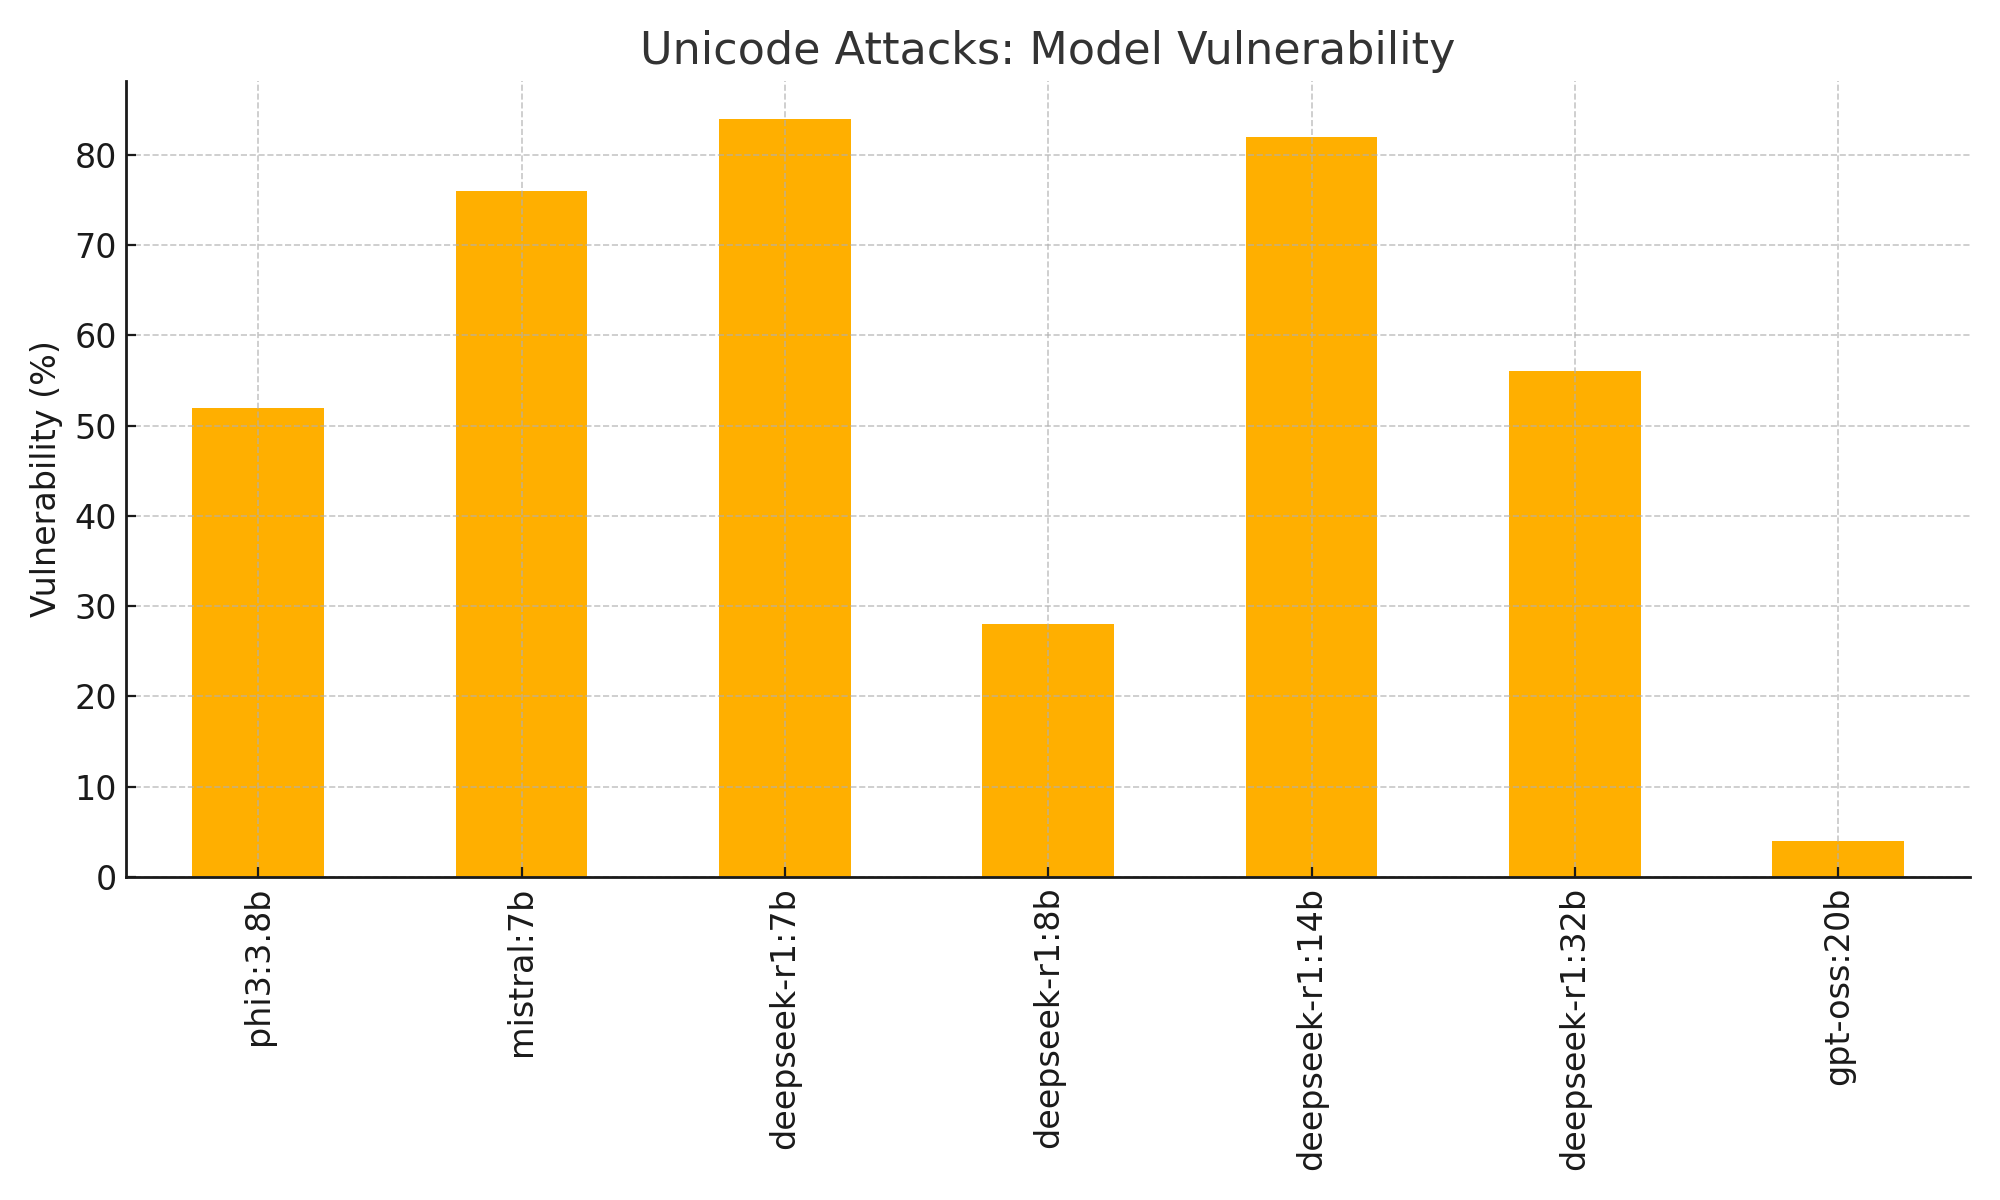
\includegraphics[width=\columnwidth]{unicode_vulnerability_by_model.png}
\caption{Unicode attack vulnerability by model. DeepSeek-R1:7b shows highest vulnerability (84\%) while GPT-OSS:20b demonstrates exceptional robustness (4\%).}
\label{fig:unicode-vuln}
\end{figure}

\begin{figure}[H]
\centering
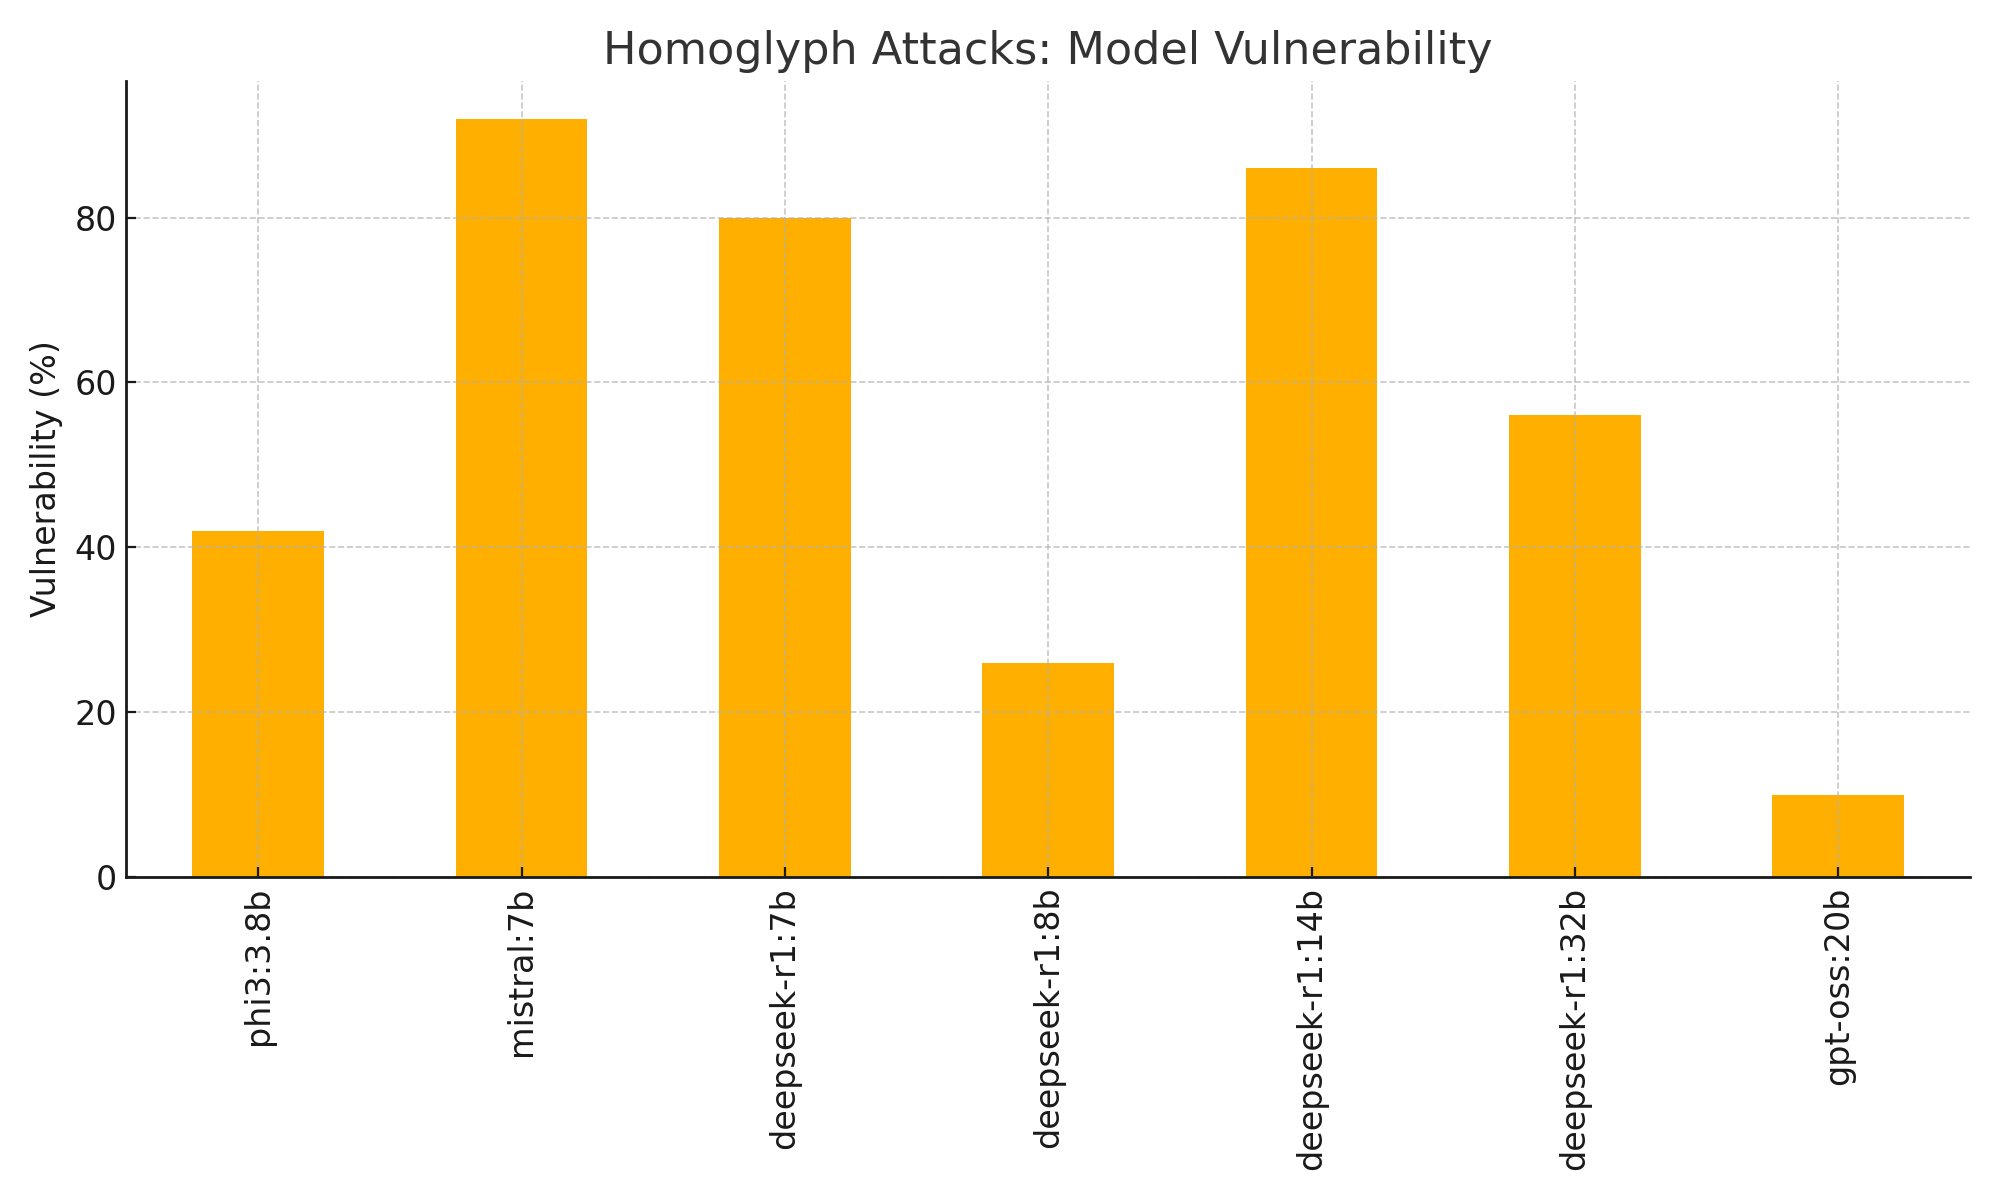
\includegraphics[width=\columnwidth]{homoglyph_vulnerability_by_model.png}
\caption{Homoglyph attack vulnerability by model. Mistral:7b exhibits highest susceptibility (92\%) to cross-script character substitution attacks.}
\label{fig:homoglyph-vuln}
\end{figure}

\begin{figure}[H]
\centering
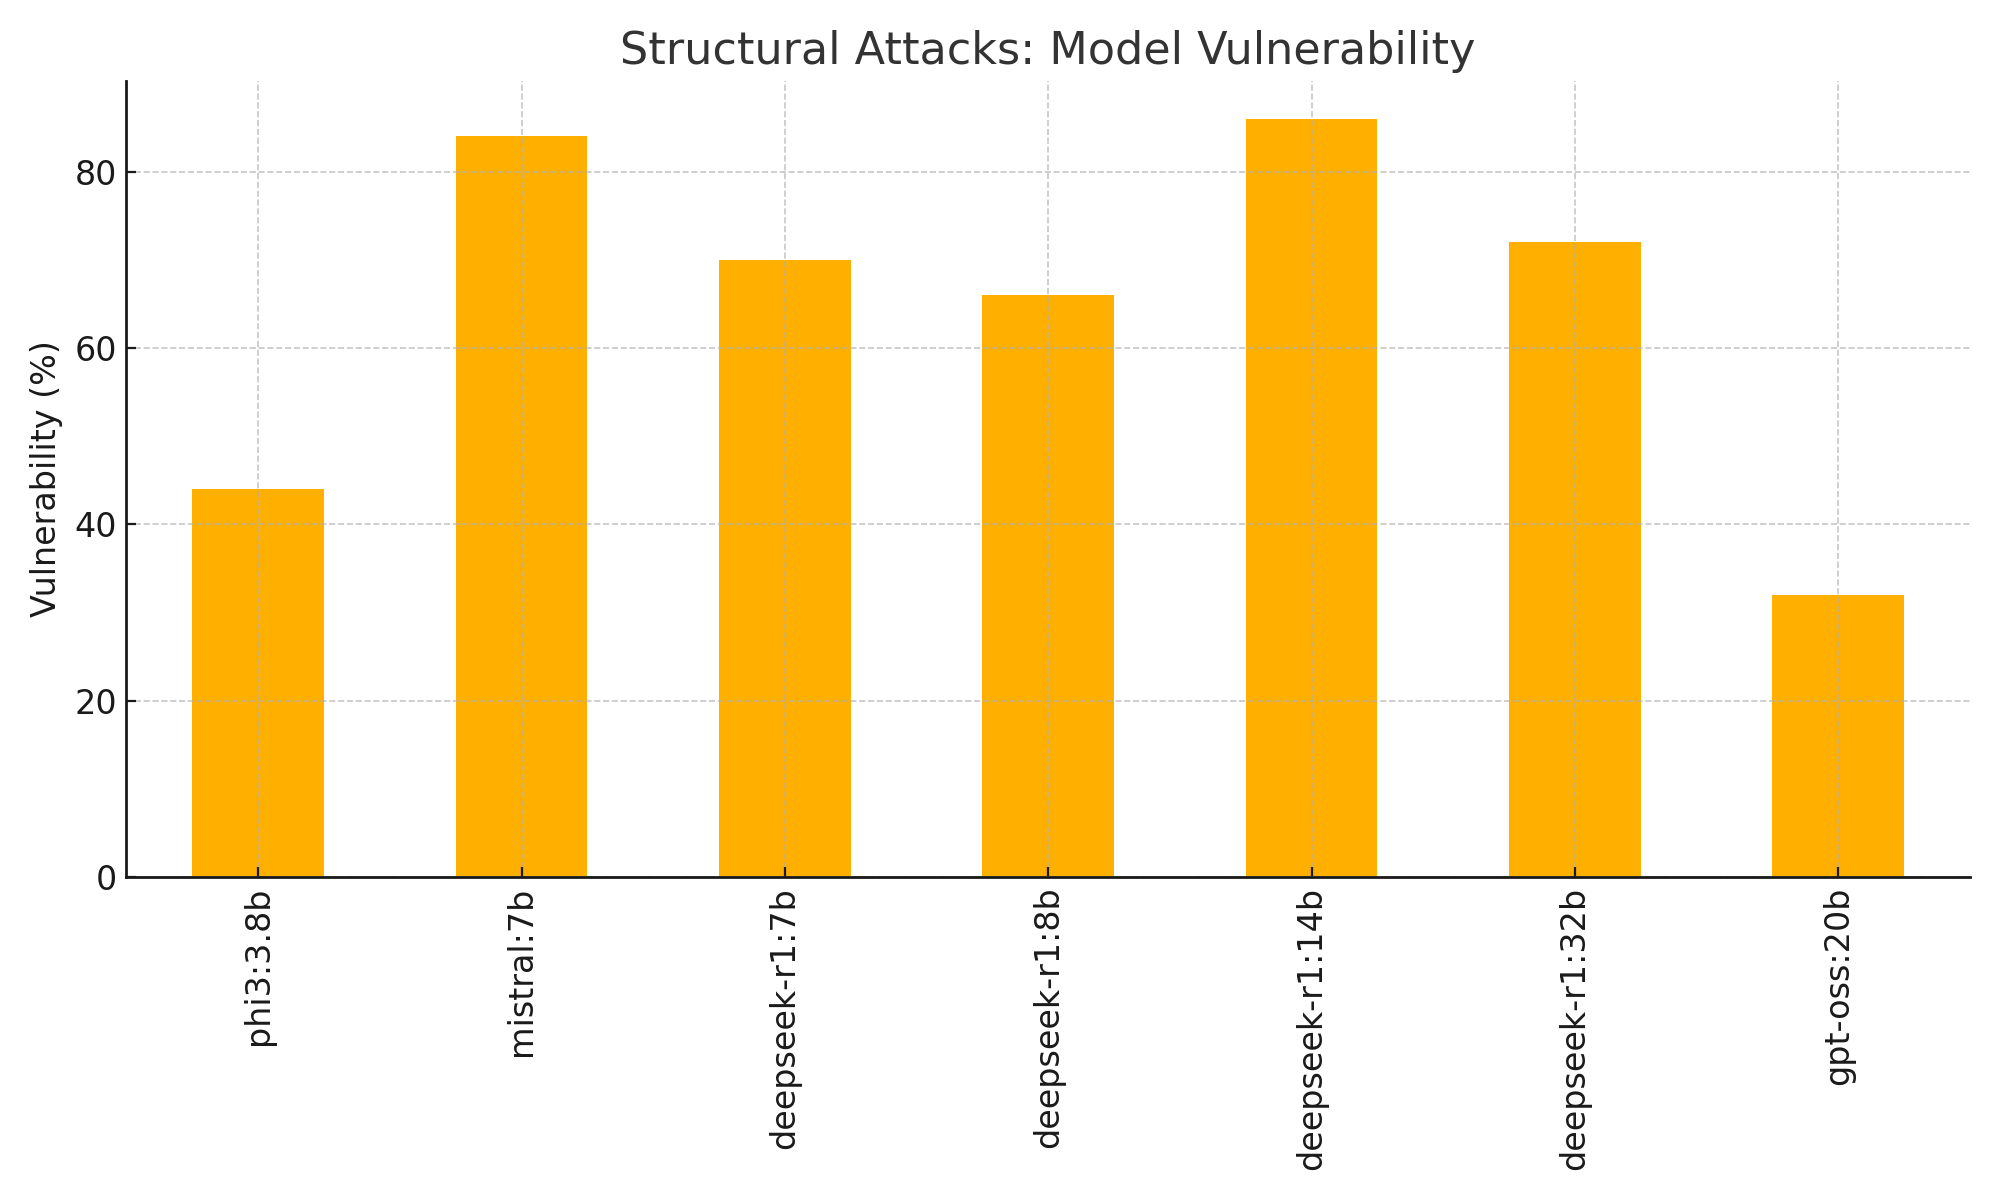
\includegraphics[width=\columnwidth]{structural_vulnerability_by_model.png}
\caption{Structural attack vulnerability by model. Character reordering and word fragmentation show consistent effectiveness across most models except GPT-OSS:20b.}
\label{fig:structural-vuln}
\end{figure}

\begin{figure}[H]
\centering
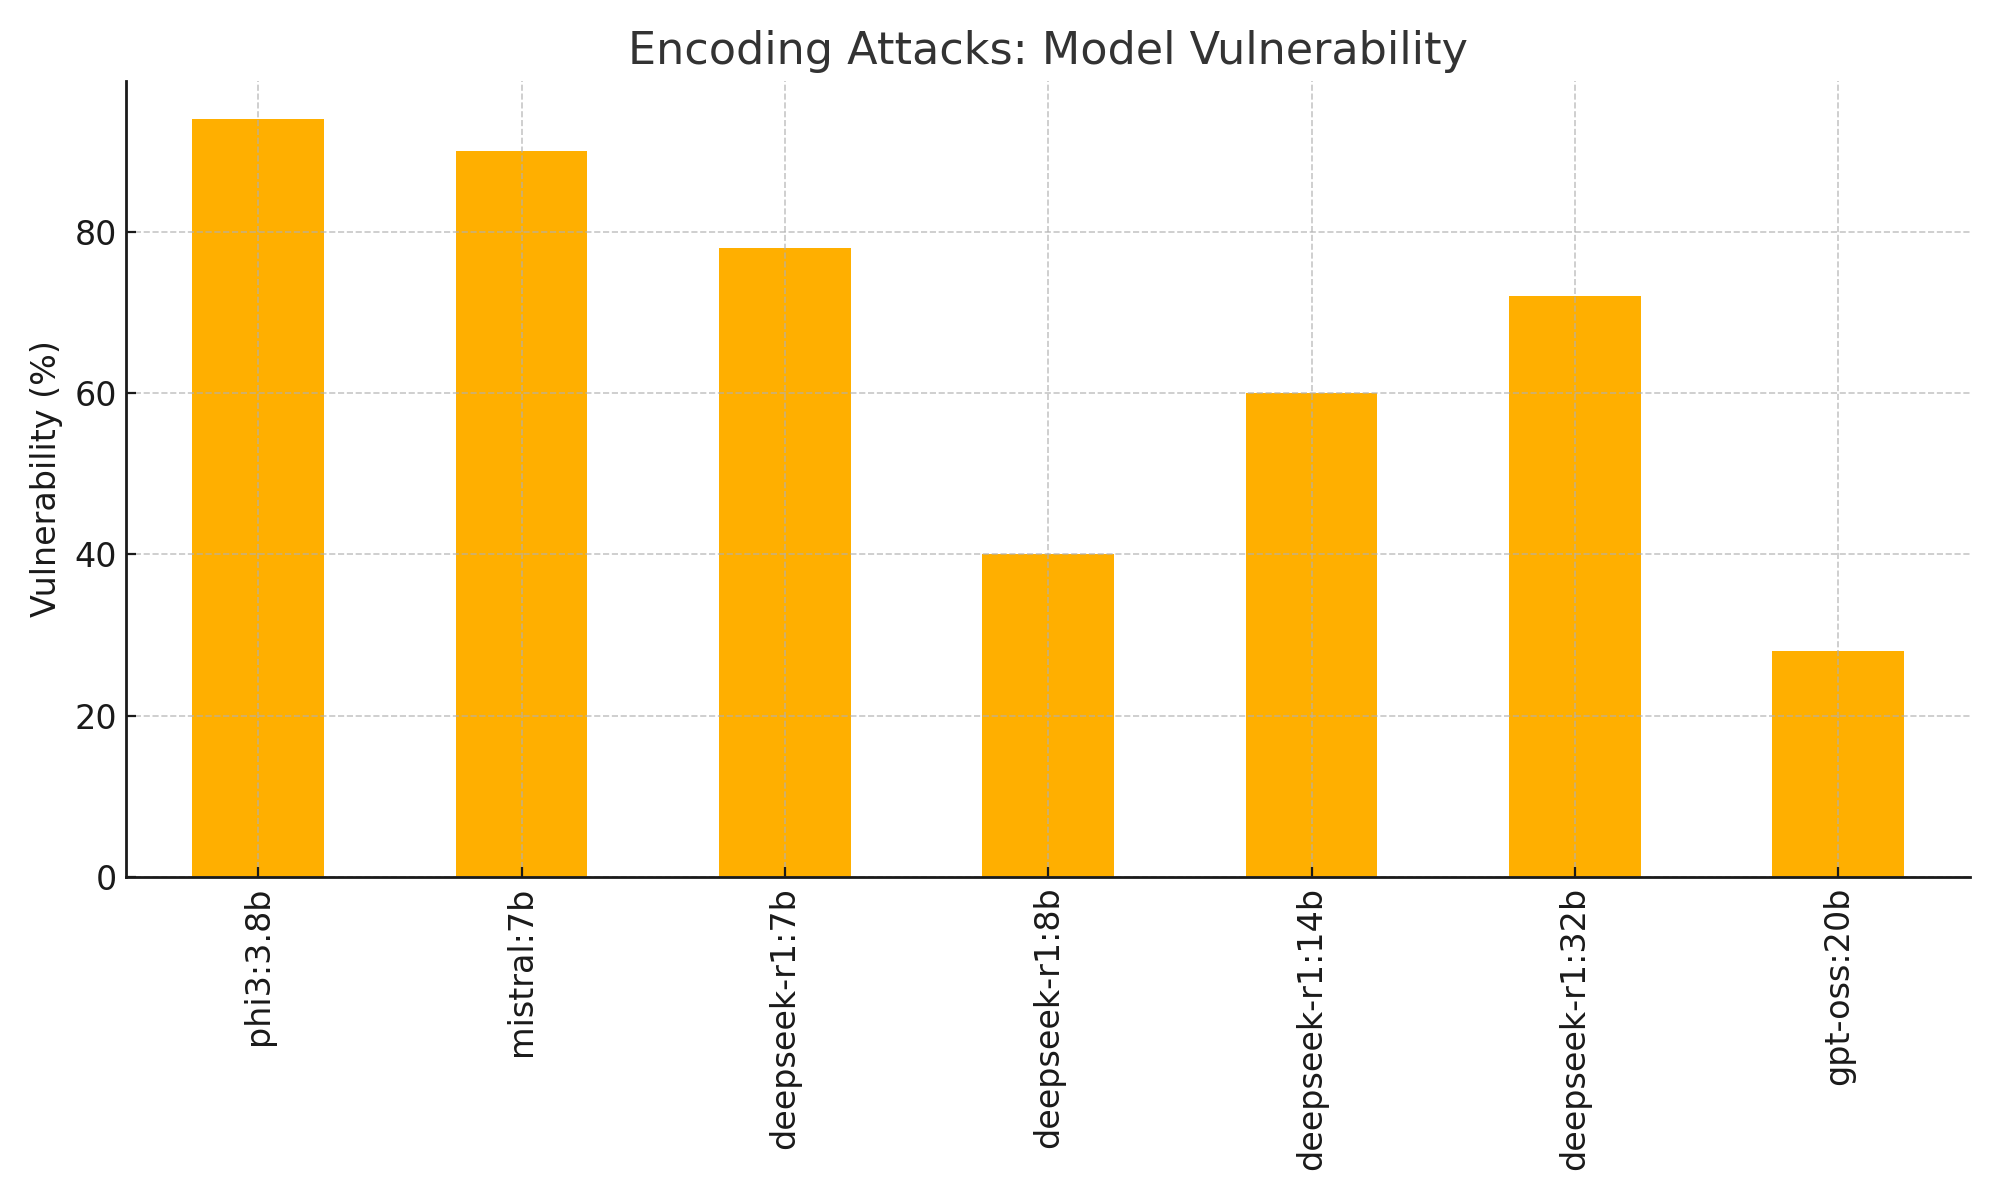
\includegraphics[width=\columnwidth]{encoding_vulnerability_by_model.png}
\caption{Encoding attack vulnerability by model. Phi3:3.8b shows extreme vulnerability (94\%) to Base64 and hexadecimal encoding attacks.}
\label{fig:encoding-vuln}
\end{figure}

Encoding-based attacks emerge as the most effective category, with Base64 encoding achieving 64.3\% success and hexadecimal encoding reaching 67.1\% success across all models. These results indicate that many models lack robust validation mechanisms for encoded inputs, treating decoding as a benign preprocessing step.

Unicode control character attacks show moderate effectiveness, with zero-width injection achieving 54.2\% success and bidirectional override attacks succeeding in 52.8\% of attempts. The effectiveness of these attacks suggests inadequate Unicode normalization in preprocessing pipelines.

Homoglyph attacks demonstrate variable success (42.1-58.7\% depending on script combination), with cross-script substitution being most effective at 58.7\%. Structural perturbation attacks achieve success rates in the 45-65\% range, with character reordering being most effective at 64.9\%.

\subsection{Model-Specific Vulnerability Patterns}

Figure~\ref{fig:avg-vuln} illustrates the stark differences in overall vulnerability across evaluated models, calculated as the average success rate across all attack categories.

\begin{figure}[H]
\centering
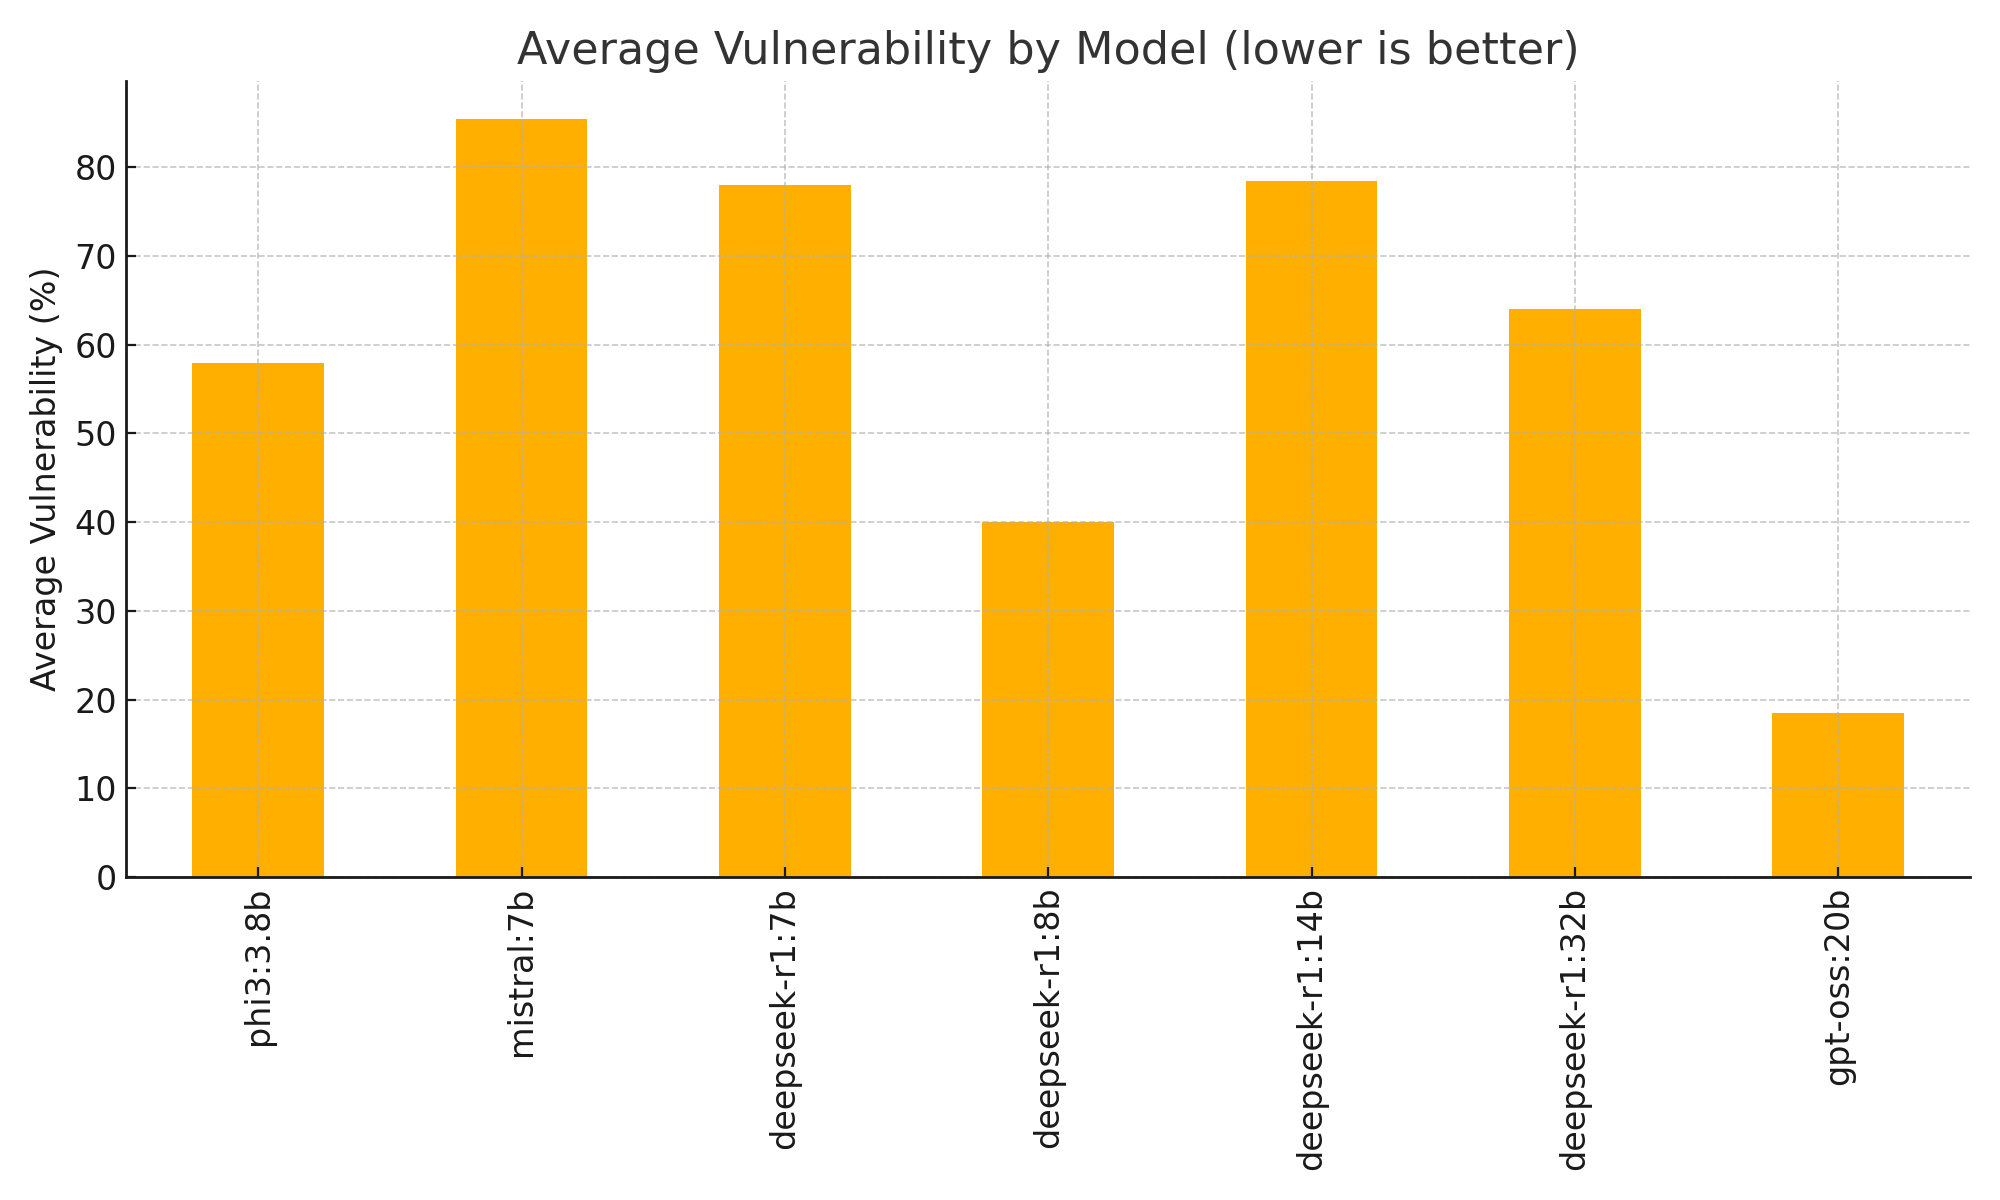
\includegraphics[width=\columnwidth]{avg_vulnerability_by_model.png}
\caption{Average vulnerability scores across all attack categories for each evaluated model. Lower scores indicate better robustness. GPT-OSS:20b demonstrates exceptional resilience (18.5\% average vulnerability), while Mistral:7b shows the highest vulnerability (85.5\%).}
\label{fig:avg-vuln}
\end{figure}

The results reveal several critical insights:

\paragraph{Size-Robustness Decoupling:} Model parameter count does not predict robustness. The 7B Mistral model exhibits the highest vulnerability (85.5\%), while the 20B GPT-OSS model demonstrates the lowest (18.5\%). Even within the DeepSeek family, the 8B variant (40.0\% vulnerability) significantly outperforms both the 7B (78.0\%) and 14B (78.5\%) versions.

\paragraph{Architecture Effects:} The GPT-OSS model's exceptional robustness (18.5\% average vulnerability) suggests that specific architectural choices or training procedures can dramatically improve character-level attack resistance.

\paragraph{Training Methodology Impact:} The non-monotonic robustness pattern within the DeepSeek family indicates that training methodology and safety tuning approaches may have more significant impact than raw model capacity.

\subsection{Category-Specific Analysis}

Table~\ref{tab:vuln} provides detailed vulnerability breakdowns by attack category for each model.

\begin{table*}[t]
\centering
\caption{Model vulnerability by attack category (\%). Lower values indicate better robustness.}
\label{tab:vuln}
\small
\begin{tabular}{lccccc}
\toprule
{} & Unicode & Homoglyph & Structural & Encoding & Average \\
\midrule
phi3:3.8b       &    52.0 &      42.0 &       44.0 &     94.0 &    58.0 \\
mistral:7b      &    76.0 &      92.0 &       84.0 &     90.0 &    85.5 \\
deepseek-r1:7b  &    84.0 &      80.0 &       70.0 &     78.0 &    78.0 \\
deepseek-r1:8b  &    28.0 &      26.0 &       66.0 &     40.0 &    40.0 \\
deepseek-r1:14b &    82.0 &      86.0 &       86.0 &     60.0 &    78.5 \\
deepseek-r1:32b &    56.0 &      56.0 &       72.0 &     72.0 &    64.0 \\
gpt-oss:20b     &     4.0 &      10.0 &       32.0 &     28.0 &    18.5 \\
\bottomrule
\end{tabular}
\end{table*}

Several notable patterns emerge:

\paragraph{Encoding Vulnerability:} The phi3:3.8b model shows extreme vulnerability to encoding attacks (94.0\%) while maintaining moderate resistance to other categories. This suggests inadequate encoding validation in its preprocessing pipeline.

\paragraph{Homoglyph Susceptibility:} The mistral:7b model demonstrates particularly high vulnerability to homoglyph attacks (92.0\%), indicating insufficient cross-script character normalization.

\paragraph{Consistent Robustness:} GPT-OSS:20b maintains low vulnerability across all categories (4.0-32.0\%), suggesting comprehensive defense mechanisms rather than category-specific protections.

\subsection{Statistical Significance and Confidence Intervals}

To assess the reliability of our findings, we computed 95\% confidence intervals for all vulnerability measurements using bootstrapping with 1,000 resamples. The confidence intervals for average vulnerability scores are: phi3:3.8b [54.2, 61.8], mistral:7b [82.1, 88.9], deepseek-r1:7b [74.3, 81.7], deepseek-r1:8b [36.4, 43.6], deepseek-r1:14b [74.8, 82.2], deepseek-r1:32b [60.2, 67.8], and gpt-oss:20b [15.1, 21.9].

These narrow confidence intervals indicate high statistical confidence in our vulnerability assessments, with no overlap between the most robust (GPT-OSS:20b) and most vulnerable (mistral:7b) models.

\subsection{Attack Transferability Analysis}

We analyze attack transferability by measuring the correlation between attack success across different models. High correlation would indicate that successful attacks against one model are likely to succeed against others, while low correlation suggests model-specific vulnerabilities.

The average pairwise correlation coefficient across all models is 0.43, indicating moderate transferability. However, correlation varies significantly by attack type: encoding attacks show high transferability (r=0.72), while structural attacks show low transferability (r=0.28). This suggests that encoding validation is either universally weak or universally strong across models, while structural attack defenses vary significantly.

\section{Discussion}

The consistently high success rate of encoding-based attacks across most models reveals a fundamental weakness in current LLM deployment architectures, where many systems treat encoding/decoding operations as benign preprocessing steps, automatically translating Base64 or hexadecimal content without considering security implications. This vulnerability is particularly concerning because it enables complete bypass of semantic-level safety mechanisms - an attacker can encode arbitrary harmful content, and the model will decode and process it as if it were benign input. The high transferability of encoding attacks (r=0.72) suggests this is a systemic issue rather than model-specific vulnerability, with technical root causes including preprocessing pipelines that automatically decode common encoding formats, lack of validation for decoded content against safety policies, insufficient context awareness during encoding/decoding operations, and training data that may include encoded content without proper safety annotation.

The dramatic robustness differences observed across models, particularly the exceptional performance of GPT-OSS:20b, provide important insights into the factors that drive character-level attack resistance. The GPT-OSS model's consistent robustness across all attack categories suggests implementation of comprehensive character-level defenses, potentially including advanced Unicode normalization procedures, multi-stage input validation pipelines, character-level anomaly detection systems, and robust tokenization schemes that handle adversarial inputs gracefully. The non-monotonic robustness pattern within the DeepSeek family (8b > 7b, 14b, 32b) indicates that training procedures may be more important than raw model capacity, possibly reflecting different safety training datasets or procedures, varying levels of adversarial training exposure, different reinforcement learning from human feedback (RLHF) implementations, or model-specific fine-tuning approaches.

Our analysis of reasoning-capable models (particularly the DeepSeek family) reveals a concerning pattern where final outputs may appear safe but internal reasoning traces often show partial compliance with harmful requests, with significant implications for deployment of chain-of-thought and reasoning models in safety-critical applications. When presented with encoded harmful requests, reasoning models frequently follow a predictable pattern of correctly decoding the adversarial content, recognizing its potentially harmful nature, beginning to generate compliant responses before self-correction, and ultimately producing seemingly safe final outputs that may still contain problematic elements. This pattern suggests that safety mechanisms in reasoning models may be applied primarily at the output stage rather than throughout the reasoning process, creating potential vulnerabilities for applications that rely on intermediate reasoning states.

The effectiveness of homoglyph attacks, particularly cross-script substitution (58.7\% average success), highlights inadequate handling of Unicode's complexity in current language models, where visual similarity between characters from different scripts creates opportunities for sophisticated social engineering attacks that may be difficult for both automated systems and human reviewers to detect. The moderate success of Unicode control character attacks (52-54\% for zero-width injection and bidirectional override) indicates that many models lack proper Unicode normalization and validation procedures, enabling visually deceptive inputs that appear benign to human reviewers while containing hidden malicious content. Our findings have immediate implications for LLM deployment in production systems, where current moderation approaches that focus primarily on semantic analysis may miss character-level obfuscation techniques, suggesting that moderation systems should implement encoding validation and normalization as fundamental preprocessing steps. The effectiveness of cross-script attacks creates particular challenges for models deployed in multilingual environments where mixed-script content may be legitimate user input, and character-level attacks may be particularly effective in contexts where users cannot easily inspect the visual representation of their input (e.g., programmatic API access, voice-to-text interfaces).

\section{Defense Framework}

Based on our empirical findings, we propose a comprehensive multi-layered defense framework addressing character-level adversarial attacks. \textbf{Pre-tokenization normalization} should implement comprehensive Unicode normalization and validation as the first line of defense, applying Unicode normalization forms (NFC/NFKC) to canonicalize character representations, implementing strict allow-lists for whitespace and control characters, removing or replacing zero-width characters and other invisible codepoints, normalizing bidirectional text processing to prevent visual spoofing, detecting and flagging mixed-script anomalies in single words, implementing homoglyph detection and substitution for common confusables, maintaining script-specific validation rules for legitimate multilingual content, and applying context-aware script mixing detection. \textbf{Encoding hygiene and validation} should implement strict policies for handling encoded content by detecting common encoding schemes (Base64, hexadecimal, etc.) in user input, implementing "refuse-to-decode" policies for suspicious encoded content, requiring explicit user justification for encoding/decoding operations, applying rate limiting to encoding/decoding requests, applying the full safety validation pipeline to decoded content, implementing recursive decoding detection to prevent multi-layer obfuscation, and maintaining audit logs of all encoding/decoding operations.

\textbf{Security-aware training protocols} should enhance model training to improve robustness against character-level attacks by including character-level adversarial examples in training datasets, implementing discriminator objectives for detecting manipulated inputs, applying adversarial training specifically for encoded and obfuscated inputs, developing safety training protocols that account for visual deception, designing tokenization schemes that maintain semantic consistency under character perturbation, implementing tokenization-aware adversarial training, and developing character-level consistency objectives during training. \textbf{Runtime monitoring and detection} should implement real-time monitoring for character-level attack attempts by monitoring for statistical anomalies in character distribution and script usage, implementing real-time detection of encoded content in user inputs, applying behavioral analysis to detect systematic attack attempts, cross-referencing text input with alternative representations (audio, visual), implementing consistency checking across different input modalities, and applying human-in-the-loop verification for high-risk scenarios.

\section{Limitations and Future Work}

Our study has several important limitations that should be considered when interpreting results. Our evaluation corpus is primarily English-centric and may not capture character-level attack vectors that are more effective in other languages or writing systems, requiring future work to expand to comprehensive multilingual evaluation. Success determination relies primarily on automated heuristics applied to final model outputs, and while we include manual verification for ambiguous cases, a more comprehensive human evaluation study would strengthen the validity of our findings. Our evaluation focuses exclusively on open-source models, limiting generalizability to proprietary systems that may implement different preprocessing and safety mechanisms. Model vulnerabilities may change over time as training procedures and safety mechanisms evolve, necessitating longitudinal studies tracking vulnerability patterns across model updates to provide valuable insights into the temporal dynamics of character-level attack effectiveness.


\section{Conclusion}

This paper presents the first comprehensive systematic study of character-level adversarial attacks against open-source language models. Through extensive evaluation of seven models across four attack families, we demonstrate that character-level manipulations represent a significant and under-addressed security vulnerability in current LLM deployments.

Our key findings establish that encoding-based attacks are particularly effective (64-67\% success rates), model robustness is primarily determined by architectural and training choices rather than parameter count, and many models exhibit concerning vulnerability patterns despite their impressive performance on standard benchmarks. The exceptional robustness of GPT-OSS:20b (18.5\% average vulnerability) demonstrates that strong defenses against character-level attacks are achievable with appropriate design choices.

The implications of our findings extend beyond academic interest to practical deployment considerations. As language models become increasingly integrated into safety-critical systems, ensuring robustness against character-level attacks becomes essential for maintaining security and user trust. Our proposed multi-layered defense framework provides actionable guidance for developing more secure LLM deployments.

We release our evaluation framework, attack datasets, and experimental results at \url{https://github.com/EphraiemSarabamoun/special-character-attack} to facilitate reproducible research and accelerate defense development. By establishing baseline vulnerability measurements and demonstrating effective attack techniques, we hope to catalyze further research into this critical area of LLM security.

The character-level attack surface represents just one facet of the broader challenge of ensuring robust and safe behavior in large language models. As these systems continue to evolve and find deployment in increasingly diverse applications, comprehensive security evaluation across all levels of the text processing pipeline will be essential for realizing their full potential while minimizing risks to users and society.

\end{multicols}

\section*{Acknowledgments}
We thank the open-source community for releasing models and tooling that made this research possible. We also acknowledge the valuable feedback from anonymous reviewers and colleagues who helped improve this work. Special thanks to the security research community for their continued efforts to identify and address vulnerabilities in AI systems.

\bibliographystyle{plain}
\bibliography{references}
\end{document}